\section{FeRAM Technology and Advances}

Doped HfO$_2$ ferroelectrics enable FeRAM and FeFET with CMOS-friendly integration \cite{boscke2011,mueller2012}. 
Recent work improves endurance and retention via stack engineering, wake-up/fatigue mitigation, and interface optimization, 
but variability and high-field reliability (e.g., TDDB) remain key concerns \cite{noheda2023,martin2020}. 
At the system level, non-volatility enables instant-on and low-power standby, complementing DRAM.

% ==== Fig.2: Write energy vs. write time (TikZ/PGFPlots) ====
\begin{figure}[!t]
\centering
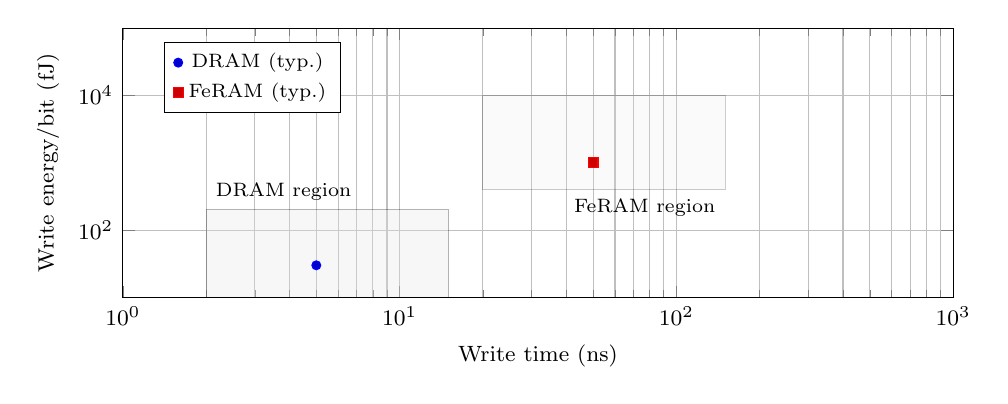
\begin{tikzpicture}
\begin{loglogaxis}[
  width=\linewidth,
  height=5.0cm,
  xlabel={Write time (ns)},
  ylabel={Write energy/bit (fJ)},
  xmin=1e0, xmax=1e3,
  ymin=1e1, ymax=1e5,
  grid=both,
  legend style={at={(0.05,0.95)},anchor=north west, font=\scriptsize},
  label style={font=\footnotesize},
  tick label style={font=\footnotesize}
]
% Typical points (conceptual)
\addplot+[only marks,mark=*,mark size=1.6pt] coordinates {(5, 30)};     
\addlegendentry{DRAM (typ.)}
\addplot+[only marks,mark=square*,mark size=1.8pt] coordinates {(50, 1000)};  
\addlegendentry{FeRAM (typ.)}

% DRAM region (conceptual)
\addplot [draw=black, fill=black!10, opacity=0.3] 
  coordinates {(2,10) (15,10) (15,200) (2,200)} -- cycle;
% FeRAM region (conceptual)
\addplot [draw=black, fill=black!10, opacity=0.2] 
  coordinates {(20,400) (150,400) (150,1e4) (20,1e4)} -- cycle;

\node[anchor=south west, font=\scriptsize] at (axis cs:2,200) {DRAM region};
\node[anchor=north east, font=\scriptsize] at (axis cs:150,400) {FeRAM region};
\end{loglogaxis}
\end{tikzpicture}
\caption{Conceptual write energy vs.\ write time. DRAM achieves lower energy at short writes; FeRAM writes cost more energy but persist without refresh.}
\label{fig:energy_speed}
\end{figure}
